\chapter{Machine Learning (ML)}

\section{A Taxonomy of Learning Problems \cite{dnn-1}} \label{A Taxonomy of Learning Problems}

\begin{enumerate}[itemsep=0.3cm]
    \item \textbf{Batch Learning}
    \begin{enumerate}
        \item In batch learning, we have access to training features and labels $\{(\mathbf{x}_1, y_1), \ldots, (\mathbf{x}_n, y_n)\}$ which we use to train a model $f(x)$. 
        
        \item Later on, we deploy this model to score new data $(x, y)$ drawn from the same distribution.

    \end{enumerate}

    \item \textbf{Online Learning}
    \begin{enumerate}
        \item the data $(x_i, y_i)$ arrives one sample at a time.

        \item assume that we first observe $x_i$ , then we need to come up with an estimate $f(x_i)$ and only once we have done this, we observe $y_i$ and with it, we receive a reward or incur a loss, given our decision.

        \item in online learning, we have the \textit{following cycle} where we are \textbf{continuously improving} our model given new observations:
        \[
            \textrm{model } f_t 
            \longrightarrow 
            \textrm{data }  \mathbf{x}_t 
            \longrightarrow 
            \textrm{estimate } f_t(\mathbf{x}_t) 
            \longrightarrow
            \textrm{observation } y_t 
            \longrightarrow 
            \textrm{loss } l(y_t, f_t(\mathbf{x}_t)) 
            \longrightarrow 
            \textrm{model } f_{t+1}
        \]

    \end{enumerate}

    \item \textbf{Bandits}
    \begin{enumerate}
        \item Bandits are a special case of Online learning.

        \item While in most learning problems we have a continuously parametrized function f where we want to learn its parameters (e.g., a deep network), in a bandit problem we only have a finite number of arms that we can pull, i.e., a finite number of actions that we can take. 

        \item It is not very surprising that for this simpler problem stronger theoretical guarantees in terms of optimality can be obtained. 

        \item This is often (confusingly) treated as if it were a distinct learning setting.

    \end{enumerate}

    \item \textbf{Control}
    \begin{enumerate}
        \item the environment remembers what we did

        \item Not necessarily in an adversarial manner but it will just remember and the response will depend on what happened before.

        \item PID (proportional-integral-derivative) controller algorithms are a popular choice there.\\
        Likewise, a user’s behavior on a news site will depend on what we showed them previously (e.g., they will read most news only once).

        \item Many such algorithms form a model of the environment in which they act so as to make their decisions appear less random. 

        \item For instance, a coffee boiler controller will observe different temperatures depending on whether it was heating the boiler previously.

    \end{enumerate}

    \item \fullref{Reinforcement Learning}
\end{enumerate}


\section{Supervised Learning \cite{drl-1}}\label{Supervised Learning}

\begin{enumerate}
    \item Supervised learning is learning from a training set of labeled examples provided by a knowledgable external supervisor. \cite{drl-1}

    \item Each example is a description of a situation together with a specification - the label - of the correct action the system should take to that situation, which is often to identify a category to which the situation belongs. \cite{drl-1}
    
    \item The object of this kind of learning is for the system to extrapolate, or generalize, its responses so that it acts correctly in situations not present in the training set. \cite{drl-1}

    
\end{enumerate}
\section{Semi-Supervised Learning}\label{Semi-Supervised Learning}



\section{Self-Supervised Learning}\label{Self-Supervised Learning}



\section{Unsupervised Learning}\label{Unsupervised Learning}


\section{Reinforcement Learning \cite{drl-1}} \label{Reinforcement Learning}

\begin{enumerate}
    \item Reinforcement learning is learning what to do - how to map situations to actions - so as to maximize a numerical reward signal.

    \item The learner is \textbf{NOT} told which actions to take, but instead must discover which actions yield the most reward by trying them.

    \item These two characteristics - \textbf{trial-and-error search} and \textbf{delayed reward} - are the two most important distinguishing features of reinforcement learning.

    \item  Although one might be tempted to think of reinforcement learning as a kind of unsupervised learning because it does not rely on examples of correct behavior, \textbf{reinforcement learning is trying to maximize a reward signal instead of trying to find hidden structure}. 
    
    \item Uncovering structure in an agent’s experience can certainly be useful in reinforcement learning, but by itself does not address the reinforcement learning problem of maximizing a reward signal.

    \item  To obtain a lot of reward, a reinforcement learning agent must prefer actions that it has tried in the past and found to be elective in producing reward. 
    
    \item But to discover such actions, it has to try actions that it has not selected before. 
    
    \item The agent has to \textbf{exploit} what it has already experienced in order to obtain reward, but it also has to \textbf{explore} in order to make better action selections in the future. 
    
    \item The dilemma is that neither exploration nor exploitation can be pursued exclusively without failing at the task. 
    
    \item The agent must try a variety of actions and progressively favor those that appear to be best. 

    \item On a \textbf{stochastic task}, each action must be tried many times to gain a reliable estimate of its expected reward.

    \item Another key feature of reinforcement learning is that it explicitly considers the \textbf{whole problem} of a \textbf{goal-directed agent} interacting with an uncertain environment.

    \item All reinforcement learning agents have explicit \textbf{goals}, can sense aspects of their \textbf{environments}, and can choose \textbf{actions} to influence their environments

    \item it is usually assumed from the beginning that the agent has to operate despite significant uncertainty about the environment it faces.

    \item  For learning research to make progress, important subproblems have to be isolated and studied, but they should be subproblems that play clear roles in complete, interactive, goal-seeking agents, even if all the details of the complete agent cannot yet be filled in.

    \item When reinforcement learning involves \textbf{supervised learning} (SEE: \fullref{Supervised Learning}), it does so for specific reasons that determine which capabilities are critical and which are not.
\end{enumerate}

\subsection{Elements of Reinforcement Learning \cite{drl-1}}\label{Elements of Reinforcement Learning}

\subsubsection{Policy ($\pi$) \cite{drl-1}}\label{RL: policy}

\begin{enumerate}
    \item A policy defines the learning agent’s way of behaving at a given time. 

    \item a policy is a \textbf{mapping} from perceived states of the environment to actions to be taken when in those states. 

    \item In some cases the policy may be a simple function or lookup table, whereas in others it may involve extensive computation such as a search process. 

    \item The policy is the core of a reinforcement learning agent in the sense that it alone is \textbf{sufficient} to determine behavior.

    
\end{enumerate}


\subsubsection{Reward \& Reward Signal \cite{drl-1}} \label{rl: reward signal}

\begin{enumerate}
    \item A reward signal defines the goal of a reinforcement learning problem.

    \item On each time step, the environment sends to the reinforcement learning agent a single number called the \textbf{reward}.

    \item The agent’s sole objective is to \textbf{maximize} the \textbf{total reward} it receives over the \textbf{long run}. 

    \item The reward signal thus defines what are the good and bad events for the agent.

    \item They are the \textbf{immediate} and defining features of the problem faced by the agent. 
    
    \item The reward signal is the primary basis for altering the policy; if an action selected by the policy is followed by low reward, then the policy may be changed to select some other action in that situation in the future.

    \item Rewards are basically given \textbf{directly} by the environment.

    
\end{enumerate}

\subsubsection{Value function \cite{drl-1}}\label{rl: Value function}

\begin{enumerate}
    \item  a value function specifies what is good in the long run.

    \item the value of a state is the total amount of reward an agent can expect to accumulate over the \textbf{future}, starting from that state.

    \item values indicate the long-term desirability of states after taking into account the states that are \textbf{likely} to follow and the rewards available in those states.

    \item \textbf{EXAMPLE}: a state might always yield a low immediate reward but still have a high value because it is regularly followed by other states that yield high rewards. Or the reverse could be true.

    \item values must be estimated and re-estimated from the sequences of observations an agent makes over its \textbf{entire lifetime}

    
\end{enumerate}

\subsubsection{Model (optional) \cite{drl-1}}\label{rl: model}
\begin{enumerate}
    \item This is something that mimics the behavior of the environment, or more generally, that allows inferences to be made about how the environment will behave.

    \item given a state and action, the model might predict the resultant next state and next reward. 
    
    \item Models are used for planning, by which we mean any way of deciding on a course of action by considering possible future situations before they are actually experienced. 
    
    \item Methods for solving reinforcement learning problems that use models and \textbf{planning} are called \textbf{model-based methods}\indexlabel{rl: model-based methods}, as opposed to simpler \textbf{model-free methods}\indexlabel{rl: model-free methods} that are explicitly trial-and-error learners - viewed as almost the opposite of planning.
\end{enumerate}



\subsection*{Note \cite{drl-1}}
\begin{enumerate}
    \item Rewards are in a sense \textbf{primary}, whereas values, as predictions of rewards, are \textbf{secondary}.

    \item Without rewards there could be no values, and the only purpose of estimating values is to achieve more reward.

    \item it is values with which we are most concerned when making and evaluating decisions. Action choices are made based on value judgments.

    \item We seek actions that bring about states of highest value, not highest reward, because these actions obtain the greatest amount of reward for us over the long run.

    
\end{enumerate}


\subsection*{Challenges \cite{drl-1}}
\begin{enumerate}
    \item[] One of the challenges that arise in reinforcement learning, and not in other kinds of learning, is the trade-off between \textbf{exploration} and \textbf{exploitation}.

    
\end{enumerate}



\subsection{Example: Tic-Tac-Toe \cite{drl-1}}

\begin{table}[H]
    \begin{minipage}{0.79\linewidth}
        \textbf{Rules}:
        \begin{enumerate}
            \item \textbf{Two players} take turns playing on a three-by-three board. 
            
            \item One player plays \textbf{X}s and the other \textbf{O}s until one player \textbf{wins} by placing three marks in a row, \textit{horizontally}, \textit{vertically}, or \textit{diagonally}, as the \textbf{X} player has in the game shown to the right. 
            
            \item If the board fills up with neither player getting three in a row, then the game is a \textbf{draw}.
        \end{enumerate}
    \end{minipage}
    \hfill
    \begin{minipage}{0.19\linewidth}
        \begin{table}[H]
            \centering
            \begin{tabular}{c|c|c}
                 X & O & O \\
                 \hline
                 O & X & X \\
                 \hline
                 && X\\
            \end{tabular}
        \end{table}
    \end{minipage}
\end{table}

\noindent
\textbf{Possible Solutions}:
\begin{enumerate}
    \item Classical “\textbf{minimax}” solution from \textit{game theory} is not correct here because it assumes a particular way of playing by the opponent. For example, a minimax player would never reach a game state from which it could lose, even if in fact it always won from that state because of incorrect play by the opponent.

    \item Classical optimization methods for sequential decision problems, such as dynamic programming, can compute an optimal solution for any opponent, but require as input a complete specification of that opponent, including the probabilities with which the opponent makes each move in each board state.
\end{enumerate}


\noindent \textbf{Resources}:
\begin{enumerate}
    \item \url{https://playtictactoe.org/}

    \item \url{https://zackakil.github.io/deep-tic-tac-toe/}

    
\end{enumerate}




\vspace{0.2cm}
\noindent \textbf{DRL-T1} 30/548 \\
\noindent \textbf{CHECK}: \fullref{Deep Reinforcement Learning (DRL)}



\section{Model Complexity \cite{dnn-1}}
\begin{enumerate}[itemsep=0.2cm]
    \item When we work with more complex models and/or fewer examples, we expect the training error to go down but the generalization gap to grow. \cite{dnn-1}

    \item In general, absent any restriction on our model class, we \textbf{CANNOT} conclude based on fitting the training data alone that our model has discovered any generalizable pattern. \cite{dnn-1}

    \item On the other hand, if our model class was not capable of fitting arbitrary labels, then it must have discovered a pattern. \cite{dnn-1}

    \item According to \textbf{Karl Popper}, a theory that can explain any and all observations is not a scientific theory at all. In short, what we want is a hypothesis that could not explain any observations we might conceivably make and yet nevertheless happens to be compatible with those observations that we in fact make. \cite{dnn-1}

    \item Often, models with more parameters are able to fit a greater number of arbitrarily assigned labels. However, this is not necessarily true. For instance, kernel methods operate in spaces with infinite numbers of parameters, yet their complexity is controlled by other means.

    \item One notion of complexity that often proves useful is the range of values that the parameters can take. A model whose parameters are permitted to take arbitrary values would be more complex.

    \item When a model is capable of fitting arbitrary labels, low training error does not necessarily imply low generalization error. However, it does not necessarily imply high generalization error either!

    \item we want to watch out for cases when our training error and validation error are both substantial but there is a little gap between them. If the model is unable to reduce the training error, that could mean that our model is too simple (i.e., insufficiently expressive) to capture the pattern that we are trying to model. Since the generalization gap $(R_\textrm{emp} - R)$ between our training and generalization errors is small, we have reason to believe that we could get away with a more complex model. This phenomenon is known as \textbf{underfitting}.

    \item When our training error is significantly lower than our validation error, indicating severe \textbf{overfitting}.

    
\end{enumerate}



\section{Model Selection \cite{dnn-1}}\label{Model Selection}

\begin{enumerate}[itemsep=0.2cm]
    \item we select our final model only after evaluating multiple models that differ in various ways (different architectures, training objectives, selected features, data preprocessing, learning rates, etc.)

    \item In principle, we should not touch our test set until after we have chosen all our hyperparameters. Were we to use the test data in the model selection process, there is a risk that we might overfit the test data. Then we would be in serious trouble. If we overfit our training data, there is always the evaluation on test data to keep us honest. But if we overfit the test data, how would we ever know?

    \item The common practice for addressing the problem of \textit{training on the test set} is to split our data three ways, incorporating a \textbf{validation set} in addition to the \textbf{training} and \textbf{test datasets}.    
\end{enumerate}


\subsection{Cross-Validation \cite{dnn-1,geeksforgeeks/cross-validation-machine-learning/}}\label{Cross-Validation}

\begin{enumerate}
    \item Cross validation is a technique used in machine learning to evaluate the performance of a model on unseen data. It involves dividing the available data into multiple folds or subsets, using one of these folds as a validation set, and training the model on the remaining folds. This process is repeated multiple times, each time using a different fold as the validation set. Finally, the results from each validation step are averaged to produce a more robust estimate of the model’s performance. \cite{geeksforgeeks/cross-validation-machine-learning/}

    \item The main purpose of cross validation is to prevent overfitting.
\end{enumerate}

\subsubsection{Holdout Validation \cite{geeksforgeeks/cross-validation-machine-learning/}} \label{Cross-Validation: Holdout Validation}

\begin{enumerate}
    \item In Holdout Validation, we perform training on the $50\%$ of the given dataset and rest $50\%$ is used for the testing purpose. 
    
    \item It’s a simple and quick way to evaluate a model. 
    
    \item The major \textbf{drawback} of this method is that we perform training on the $50\%$ of the dataset, it may possible that the remaining $50\%$ of the data contains some important information which we are leaving while training our model i.e. \textbf{higher bias}.

\end{enumerate}


\subsubsection{LOOCV (Leave One Out Cross Validation) \cite{geeksforgeeks/cross-validation-machine-learning/}} \label{Cross-Validation: LOOCV (Leave One Out Cross Validation)}

\begin{enumerate}
    \item In this method, we perform training on the whole dataset but leaves only one data-point of the available dataset and then iterates for each data-point. 
    
    \item In LOOCV, the model is trained on $n-1$ samples and tested on the one omitted sample, repeating this process for each data point in the dataset.

    \item An \textbf{advantage} of using this method is that we make use of all data points and hence it is \textbf{low bias}.

    \item The major \textbf{drawback} of this method is that it leads to \textbf{higher variation} in the testing model as we are testing against one data point. If the data point is an outlier it can lead to higher variation. 
    
    \item Another \textbf{drawback} is it takes a \textbf{lot of execution time} as it iterates over ‘the number of data points’ times.
\end{enumerate}


\subsubsection{Stratified Cross-Validation \cite{geeksforgeeks/cross-validation-machine-learning/}} \label{Cross-Validation: Stratified Cross-Validation}

\begin{enumerate}
    \item It is a technique used in machine learning to ensure that each fold of the cross-validation process maintains the same class distribution as the entire dataset. 
    
    \item This is particularly important when dealing with \textbf{imbalanced datasets}, where certain classes may be underrepresented.

\end{enumerate}

\noindent
\textbf{Steps:}
\begin{enumerate}
    \item The dataset is divided into $k$ folds while maintaining the proportion of classes in each fold.
    
    \item During each iteration, one-fold is used for testing, and the remaining folds are used for training.

    \item The process is repeated $k$ times, with each fold serving as the test set exactly once.

\end{enumerate}



\subsubsection{$K$-Fold Cross Validation \cite{geeksforgeeks/cross-validation-machine-learning/}} \label{Cross-Validation: K-Fold Cross Validation}

\begin{table}[H]
    \begin{minipage}{0.38\linewidth}
        \begin{figure}[H]
            \centering
            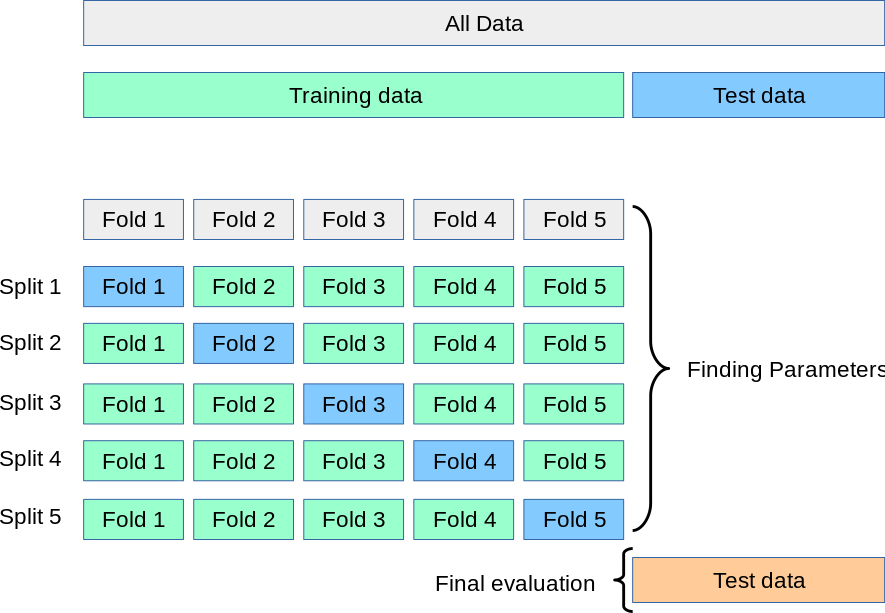
\includegraphics[width=\linewidth, height=5cm, keepaspectratio]{Pictures/ai-ml/grid_search_cross_validation.png}
        \end{figure}
    \end{minipage}
    \hfill
    \begin{minipage}{0.58\linewidth}
        \begin{enumerate}
            \item In $K$-Fold Cross Validation, we split the dataset into $k$ number of subsets (known as folds) then we perform training on the all the subsets but leave one $(k-1)$ subset for the evaluation of the trained model. 
            
            \item  We iterate $k$ times with a different subset reserved for testing purpose each time.
        
        \end{enumerate}
    \end{minipage}
\end{table}


\section{Fairness, Accountability, and Transparency in Machine Learning} \label{Fairness, Accountability, and Transparency in Machine Learning}

\begin{enumerate}
    \item it is important to remember that when you deploy machine learning systems you are not merely optimizing a predictive model—you are typically providing a tool that will be used to (partially or fully) automate decisions. 
    
    \item These technical systems can impact the lives of individuals who are subject to the resulting decisions. 
    
    \item The leap from considering predictions to making decisions raises not only new technical questions, but also a slew of ethical questions that must be carefully considered.

    \item Overlooking foreseeable risks to the welfare of a subpopulation could cause us to administer inferior care. 
    
    \item Moreover, once we contemplate decision-making systems, we must step back and reconsider how we evaluate our technology. 
    
    \item Among other consequences of this change of scope, we will find that accuracy is seldom the right measure.\\
    When translating predictions into actions, we will often want to take into account the potential cost sensitivity of erring in various ways.

    \item If one way of misclassifying an image could be perceived as a racial sleight of hand, while misclassification to a different category would be harmless, then we might want to adjust our thresholds accordingly, accounting for societal values in designing the decision-making protocol.

    \item \textbf{Example}: If we are deploying a medical diagnostic system, we need to know for which populations it may work and for which it may not.

    \item The various mechanisms by which a model’s predictions become coupled to its training data are unaccounted for in the modeling process. This can lead to what researchers call \textbf{runaway feedback loops}\indexlabel{runaway feedback loops}.

    
\end{enumerate}




\section*{SEE}

\begin{enumerate}
    \item \fullref{Supervised Learning VS Unsupervised Learning VS Reinforcement Learning}
\end{enumerate}








